
\vspace{-0.4cm}
\section*{Model}

We consider a Kesten process $X_n$ that models spine size dynamics. A given spine size $X_n$ at time step $n$ is updated as
%
\begin{align}
  X_{n+1} = a_n X_n + b_n, \label{eq:kesten}
\end{align}
%
where both $a_n$ and $b_n$ are drawn randomly at each time step from a normal distribution, $a_n \sim \mathcal{N}(\mu_a, \sigma_a^2)$ and $b_n \sim \mathcal{N}(\mu_b, \sigma_b^2)$. To model synapse growth and pruning processes, we consider a population of $N$ synapses. Each synapse has a random time $T_{\mathrm{init}}$, uniformly distributed in $[0,T_{\text{max}}]$, at which it is initialized with size $X_0$. The synaptic spine size $X_t$ then evolves according to \eqref{eq:kesten}.

\medskip

The lifetime of the synapse is the number of time steps from $T_{\text{init}}$ until for the first time $X_t < X_{\mathrm{prune}}$, where $X_{\mathrm{prune}}$ is a fixed parameter smaller than $X_0$ for the population. In this event the synapse gets pruned and a new synapse with size $X_0$ is inserted in the network (Fig.~\ref{fig:km}). In the case that $X_t$ doesn't fall below $X_{\mathrm{prune}}$ until $T_{\text{max}}$, the lifetime is recorded as $T=T_{\text{max}}-T_{\text{init}}$. At the end of the simulation the sizes $X_{T_{\text{max}}}$ are recorded for all $N$ synapses.

\begin{center}\vspace{1cm}
  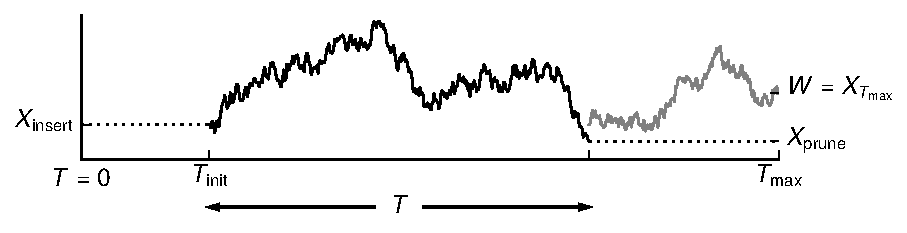
\includegraphics[width=0.95\columnwidth]{%
    figures/abstract_fig.pdf}
  %% /home/fh/sci/lab/syn_lt/kesten_model/note_x/km_ca_rts_dd/img/abstract_fig.png}
  \captionof{figure}{Adapted Kesten simulation model allows the tracking of lifetimes and size distributions}
  \label{fig:km}
\end{center}\vspace{1.4cm}
